\documentclass[11pt]{article}
% ---------------------------------------------------------------------------
% Project One, ECO1465 Applied Causal Machine Learning
% Compiled by 00_master/00_master.py (or: cd 03_output/paper && pdflatex main && pdflatex main)
% Tables are \input from ../tables, figures from ../figures.
% ---------------------------------------------------------------------------
\usepackage[margin=1in]{geometry}
\usepackage[T1]{fontenc}
\usepackage{mathptmx}
\renewcommand{\ttdefault}{pcr}
\usepackage{amsmath,booktabs,threeparttable,graphicx,float,caption,subcaption,setspace,enumitem}
\usepackage[authoryear,round]{natbib}
\usepackage{xcolor}
\usepackage[colorlinks=true,linkcolor=blue!60!black,citecolor=blue!60!black,urlcolor=blue!60!black]{hyperref}
\captionsetup{font=small,labelfont=bf}
\setlength{\parskip}{3pt}
\graphicspath{{../figures/}}
\newcommand{\tabpath}{../tables}
\setstretch{1.08}

\begin{document}

\begin{center}
{\Large\textbf{Do Local Chiefs Grant More Discretionary Tax Exemptions?\\[2pt]
Evidence from a Randomized Tax Collection Experiment in Kananga, D.R.\ Congo}}\\[8pt]
\textbf{Name:} Tsu Ning Tsao \qquad \textbf{Student Number:} 1012713137
\end{center}

\begin{abstract}
\noindent Governments in weak states increasingly hand tax collection to local elites, who know their neighbours but also have room to favour them. I use the randomized 2018 property-tax campaign in Kananga \citep{balan2022} to ask whether city chiefs, compared with state collectors, grant more exemptions that the law does not allow. Linking collectors' exemption records to the owner's age and sex, I find that chiefs record 4.8 percentage points more old-age exemptions, and that old-age exemptions given to owners below the legal age of 55 almost double (1.4\% to 2.5\%, $p=0.01$, randomization-inference $p=0.01$). Yet the total exemption rate among owners under 55 barely moves, because chiefs record fewer widow exemptions at the same time; an exemption measure that does not rely on the stated reason shows no increase. Ridge, Lasso and tree-based models find no covariate, including co-ethnicity with the chief, along which the effect of chiefs varies. Chiefs relabel exemptions more than they hand out new ones.
\end{abstract}

% ===========================================================================
\section{Introduction}
% ===========================================================================

Low-income states raise little tax, and a common response is to borrow the capacity of people who already know the tax base \citep{besley2009,besley2014}. Village heads target transfers in Indonesia \citep{alatas2012}, chiefs allocate subsidies in Malawi \citep{basurto2020}, and in the D.R.\ Congo city chiefs collected the property tax in a randomized experiment and raised compliance by 3.2 percentage points over state agents \citep{balan2022}. The cost of this delegation is discretion. Local elites can use what they know to enforce the law, or to favour kin, co-ethnics and clients \citep{acemoglu2014,anderson2015,baldwin2016}. A tax exemption is a particularly convenient favour: it costs the chief nothing, leaves no cash trail, and is hard for the state to audit.

The main research question is whether replacing state collectors with neighbourhood chiefs increases tax exemptions that the law does not justify, and for which households the effect is larger. Congolese law exempts owners aged 55 or older, widows, state pensioners and disabled owners. I call an exemption discretionary when the reason the collector recorded contradicts the owner's own traits: an ``old-age'' exemption for an owner under 55, or a ``widow'' exemption for a male owner. I then ask whether any increase is concentrated among owners who share the chief's ethnicity, who are close to the age threshold, or whose relatives work for the state.

This question sits between two literatures that rarely meet. Work on decentralized targeting finds that local leaders use better information and target about as well as formulas \citep{alatas2012,basurto2020,bardhan2006}, while work on corruption finds that agents with discretion leak resources to themselves and their networks \citep{olken2007,olken2012,khan2016} and favour co-ethnics \citep{burgess2015,fisman2017}. \citet{balan2022} speak to both: chiefs collect more bribes (1.8 points) but exempt the elderly more often, which they read as rule-following, and they report no co-ethnic bias in exemptions. Their test compares the share exempted. I add a test of the \emph{legal basis} of each exemption, using the owner's age and sex from an independent survey, and I find a pattern their average hides: chiefs give more old-age exemptions to owners who are too young for them, but take an equal number of widow exemptions away from the same young owners. A count of exemptions misses this re-labelling, and a count of reasons overstates the favours. My second addition is methodological: I search for heterogeneity with penalized regressions and tree ensembles \citep{wager2018,athey2019} instead of a few interactions chosen in advance.

Identification comes from the experiment. Neighbourhoods were randomly assigned to chief (Local) or state (Central) collection within strata, so the Local--Central difference in exemptions is the causal effect of chief collection, with no instrument needed \citep{balan2022}. The two assumptions that need work are SUTVA and selection into the sample: only half of the properties have a recorded exemption decision, and the owner-linked sample is selected after treatment. I show that recording rates do not differ by arm, that neighbours' assignment does not affect exemptions, and that the main result survives a sample that does not condition on the collector recording a decision.

The results are as follows. In the replication sample, chiefs raise exemptions by 3.9 points over a Central mean of 26.6\%, all through old-age exemptions. In the owner-linked sample, old-age exemptions rise by 4.8 points and old-age exemptions for owners under 55 rise by 1.1 points (82\% of the Central mean), a result that holds at cut-offs of 50, 60 and 65, with covariates, with a logit, under randomization inference and after post-double-selection Lasso. But widow exemptions fall by 2.7 points, the total exemption rate rises by an insignificant 1.9 points, and exemptions of men under 55 who are not pensioners or disabled rise by an insignificant 0.6 points. No interaction is significant, Lasso sets all of them to zero, and the random forest and boosting barely use the treatment. Section~\ref{sec:data} describes the data, Section~\ref{sec:id} the identification checks, Section~\ref{sec:results} the results and Section~\ref{sec:conc} concludes.

% ===========================================================================
\section{Data and Summary Statistics}\label{sec:data}
% ===========================================================================

\paragraph{Source.} The data come from the 2018 property-tax campaign that the provincial government of Kasa\"i-Central ran with researchers in Kananga, the province's capital, and are distributed in the replication package of \citet{balan2022} (AEA registry AEARCTR-0003308). The city's 356 neighbourhoods were randomly assigned to four collection arms; I use the 221 assigned to Central (110) or Local (111, including one Central$\times$Local neighbourhood that was implemented as Local). Four sources are combined at the property level. The \emph{registration} data were entered by collectors on tablets during the door-to-door register (June--December 2018) and record, for each property, whether the collector declared it exempt and the stated reason. The \emph{tax roll and receipts} come from handheld receipt printers. The \emph{midline survey}, run by independent enumerators mostly between November 2018 and February 2019, records the owner's age, sex, tribe and job, and an enumerator's own judgement of whether the property should be exempt. The \emph{chief survey} used for randomization (December 2017--May 2018) records the tribe of every neighbourhood chief before assignment.

\paragraph{Variables and samples.} The unit is the property. The treatment $D$ is $\text{Local}_j=1$ if neighbourhood $j$ was assigned to chief collection. The main outcomes are 0/1 indicators for being exempted, for each stated reason, and for discretionary exemptions. A reason-free outcome, ``no basis'', flags any exemption of a man under 55 who is not exempted as a pensioner or disabled. Controls $X$ are pre-determined owner traits (age, sex, Luluwa, own and relative state employment, employment, wall quality, log predicted property value from the authors' machine-learning estimates, distance to the city centre) and co-ethnicity with the chief, which compares the owner's tribe with the chief's tribe in the pre-randomization survey and is therefore defined in both arms. Of 28,872 properties in the 221 neighbourhoods, 14,381 have a recorded exemption decision (the \emph{registered sample}) and 6,282 of these also have the owner's age and sex (the \emph{owner-linked sample}, 204 neighbourhoods).

\input{\tabpath/table1_sumstats.tex}

\paragraph{What the summary statistics show.} Table~\ref{tab:sumstats} contains most of the story. In the registered sample 28.6\% of properties are exempt, and almost all exemptions are for old age (14.3\%) or widowhood (11.4\%). Exemptions are far more common than tax payments (8\% of properties pay) or bribes (1.4\%), so they are the largest margin of discretion collectors have. Local neighbourhoods exempt more (31.0\% vs 26.4\%), and the gap is almost all old age (16.2\% vs 12.6\%), as \citet{balan2022} report. Panel B shows the new fact. Among owner-linked properties, old-age exemptions for owners under 55 are 1.4\% in Central and 2.6\% in Local, while widow exemptions for male owners go the other way (2.6\% vs 1.5\%). The reason-free measure is almost identical across arms (2.7\% vs 3.0\%). The numbers to watch are therefore not the level of exemptions but the mix of reasons.

\begin{figure}[!htbp]\centering
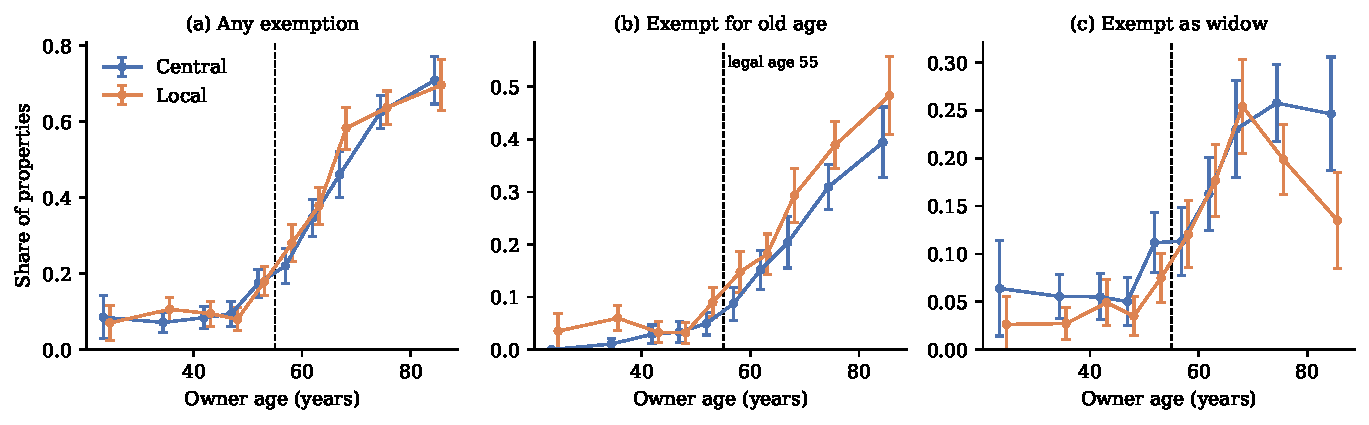
\includegraphics[width=\textwidth]{fig1_exempt_by_age.pdf}
\caption{Exemptions by owner age and arm (owner-linked sample, 95\% CI). The dashed line marks the legal old-age threshold of 55.}\label{fig:age}
\end{figure}

Figure~\ref{fig:age} plots the three exemption rates against the owner's age. Panel (a) shows that collectors in both arms follow the age rule: exemption rates are flat at about 10\% below 50 and rise steeply after 55. The Local and Central lines are almost on top of each other at every age, so chiefs do not exempt young owners more often. Panels (b) and (c) show why the reason-based measure moves anyway. Below 55, Local old-age exemptions sit above the Central line (5.5\% vs 2.9\% for owners under 55) while Local widow exemptions sit below it (4.6\% vs 6.9\%). Above 70, Local collectors record far fewer widows and far more elderly owners. Young owners in Local neighbourhoods are not exempted more; they are exempted under a different label. Most of the paper is about whether this pattern is causal and robust.

\paragraph{Data limitations and cleaning.} Three limitations matter. First, the exemption decision is missing for half of the properties, and the share recorded ranges from 2\% to 100\% across neighbourhoods, which points to collectors' data-entry habits; the recording rate does not differ by arm (Table~\ref{tab:balance}, Panel C). Second, owner age is reported by the midline respondent, and 38\% of ages are given as five-year bands, which I set to the band's mid-point as the authors do; the result holds when I drop them. Third, widowhood is not observed, so a widow exemption for a woman cannot be verified and ``widow, male'' is a lower bound on discretionary widow exemptions. I rebuild the authors' data in Python, reproduce their estimates exactly (Table~\ref{tab:replication}), and do all cleaning in one script; Appendix~\ref{app:data} lists the steps. A neighbourhood ``transport cost'' variable in the package records campaign costs, which depend on who collects, so I exclude it from balance tests and models.

% ===========================================================================
\section{Empirical Strategy and Identification}\label{sec:id}
% ===========================================================================

\paragraph{Specification.} For property $i$ in neighbourhood $j$ of stratum $s$, I estimate
\begin{equation}\label{eq:ate}
Y_{ij} = \alpha + \beta\, \text{Local}_j + \gamma_{s(j)} + \mu_{h(i)} + \tau_{t(j)} + \varepsilon_{ij},
\end{equation}
where $\gamma_s$ are randomization-stratum fixed effects, $\mu_h$ house-type fixed effects and $\tau_t$ two-month campaign-period fixed effects, exactly as in Table A9 of \citet{balan2022}. Standard errors are clustered by neighbourhood, the level of randomization. Because $\text{Local}_j$ is randomly assigned within strata, $\beta$ is the average effect of assigning chief collection on the probability that a property receives a given exemption. It is an intention-to-treat effect only in name: compliance with assignment was complete. Adding pre-determined controls $X_i'\theta$ should not change $\beta$ but can make it more precise. For heterogeneity, I add a moderator $M_i$ and its interaction,
\begin{equation}\label{eq:het}
Y_{ij} = \alpha + \beta\, \text{Local}_j + \theta M_i + \delta\, (\text{Local}_j \times M_i) + \gamma_{s} + \mu_{h} + \tau_{t} + \varepsilon_{ij},
\end{equation}
where $\delta$ measures how much more chiefs exempt owners with $M_i=1$. Since $M_i$ is pre-determined and $\text{Local}_j$ is random, $\delta$ is causal for the subgroup comparison but not for $M$ itself.

\paragraph{DAGs.} Figure~\ref{fig:dags} draws three causal graphs. In DAG~1 the only parents of Local are the coin flip and the stratum. Owner traits cause exemptions directly and through unobserved widowhood and the house band, and co-ethnicity depends on the owner's tribe and on geography, but none of these arrows enters $D$. The only back-door path, $D \leftarrow \text{stratum} \rightarrow Y$, is closed by stratum fixed effects, so equation~\eqref{eq:ate} identifies $\beta$ without conditioning on $X$. DAG~2 shows what would go wrong outside the experiment. If the government chose to delegate in older, settled neighbourhoods, owner age would cause both $D$ and $Y$, opening $D\leftarrow S\rightarrow Y$, $D\leftarrow S\rightarrow \text{Widowed}\rightarrow Y$ and $D\leftarrow S\rightarrow \text{Employment}\rightarrow Y$. Age alone blocks all three, which is why the age controls in Panel B of Table~\ref{tab:ate} matter once selection into the sample is in doubt. DAG~3 is about what not to control for. The chief's knowledge and discretion ($M$) and the stated reason ($L$) are both caused by $D$; conditioning on the stated reason would remove the very re-labelling channel I study. The endline co-ethnic-bias question ($C$) is a collider on $D\rightarrow C\leftarrow U\rightarrow Y$, where $U$ is a personal tie to the chief, so conditioning on it would open a non-causal path. I therefore measure co-ethnicity with the pre-randomization chief survey rather than with the endline question.

\begin{figure}[!htbp]\centering
\begin{subfigure}{0.46\textwidth}\centering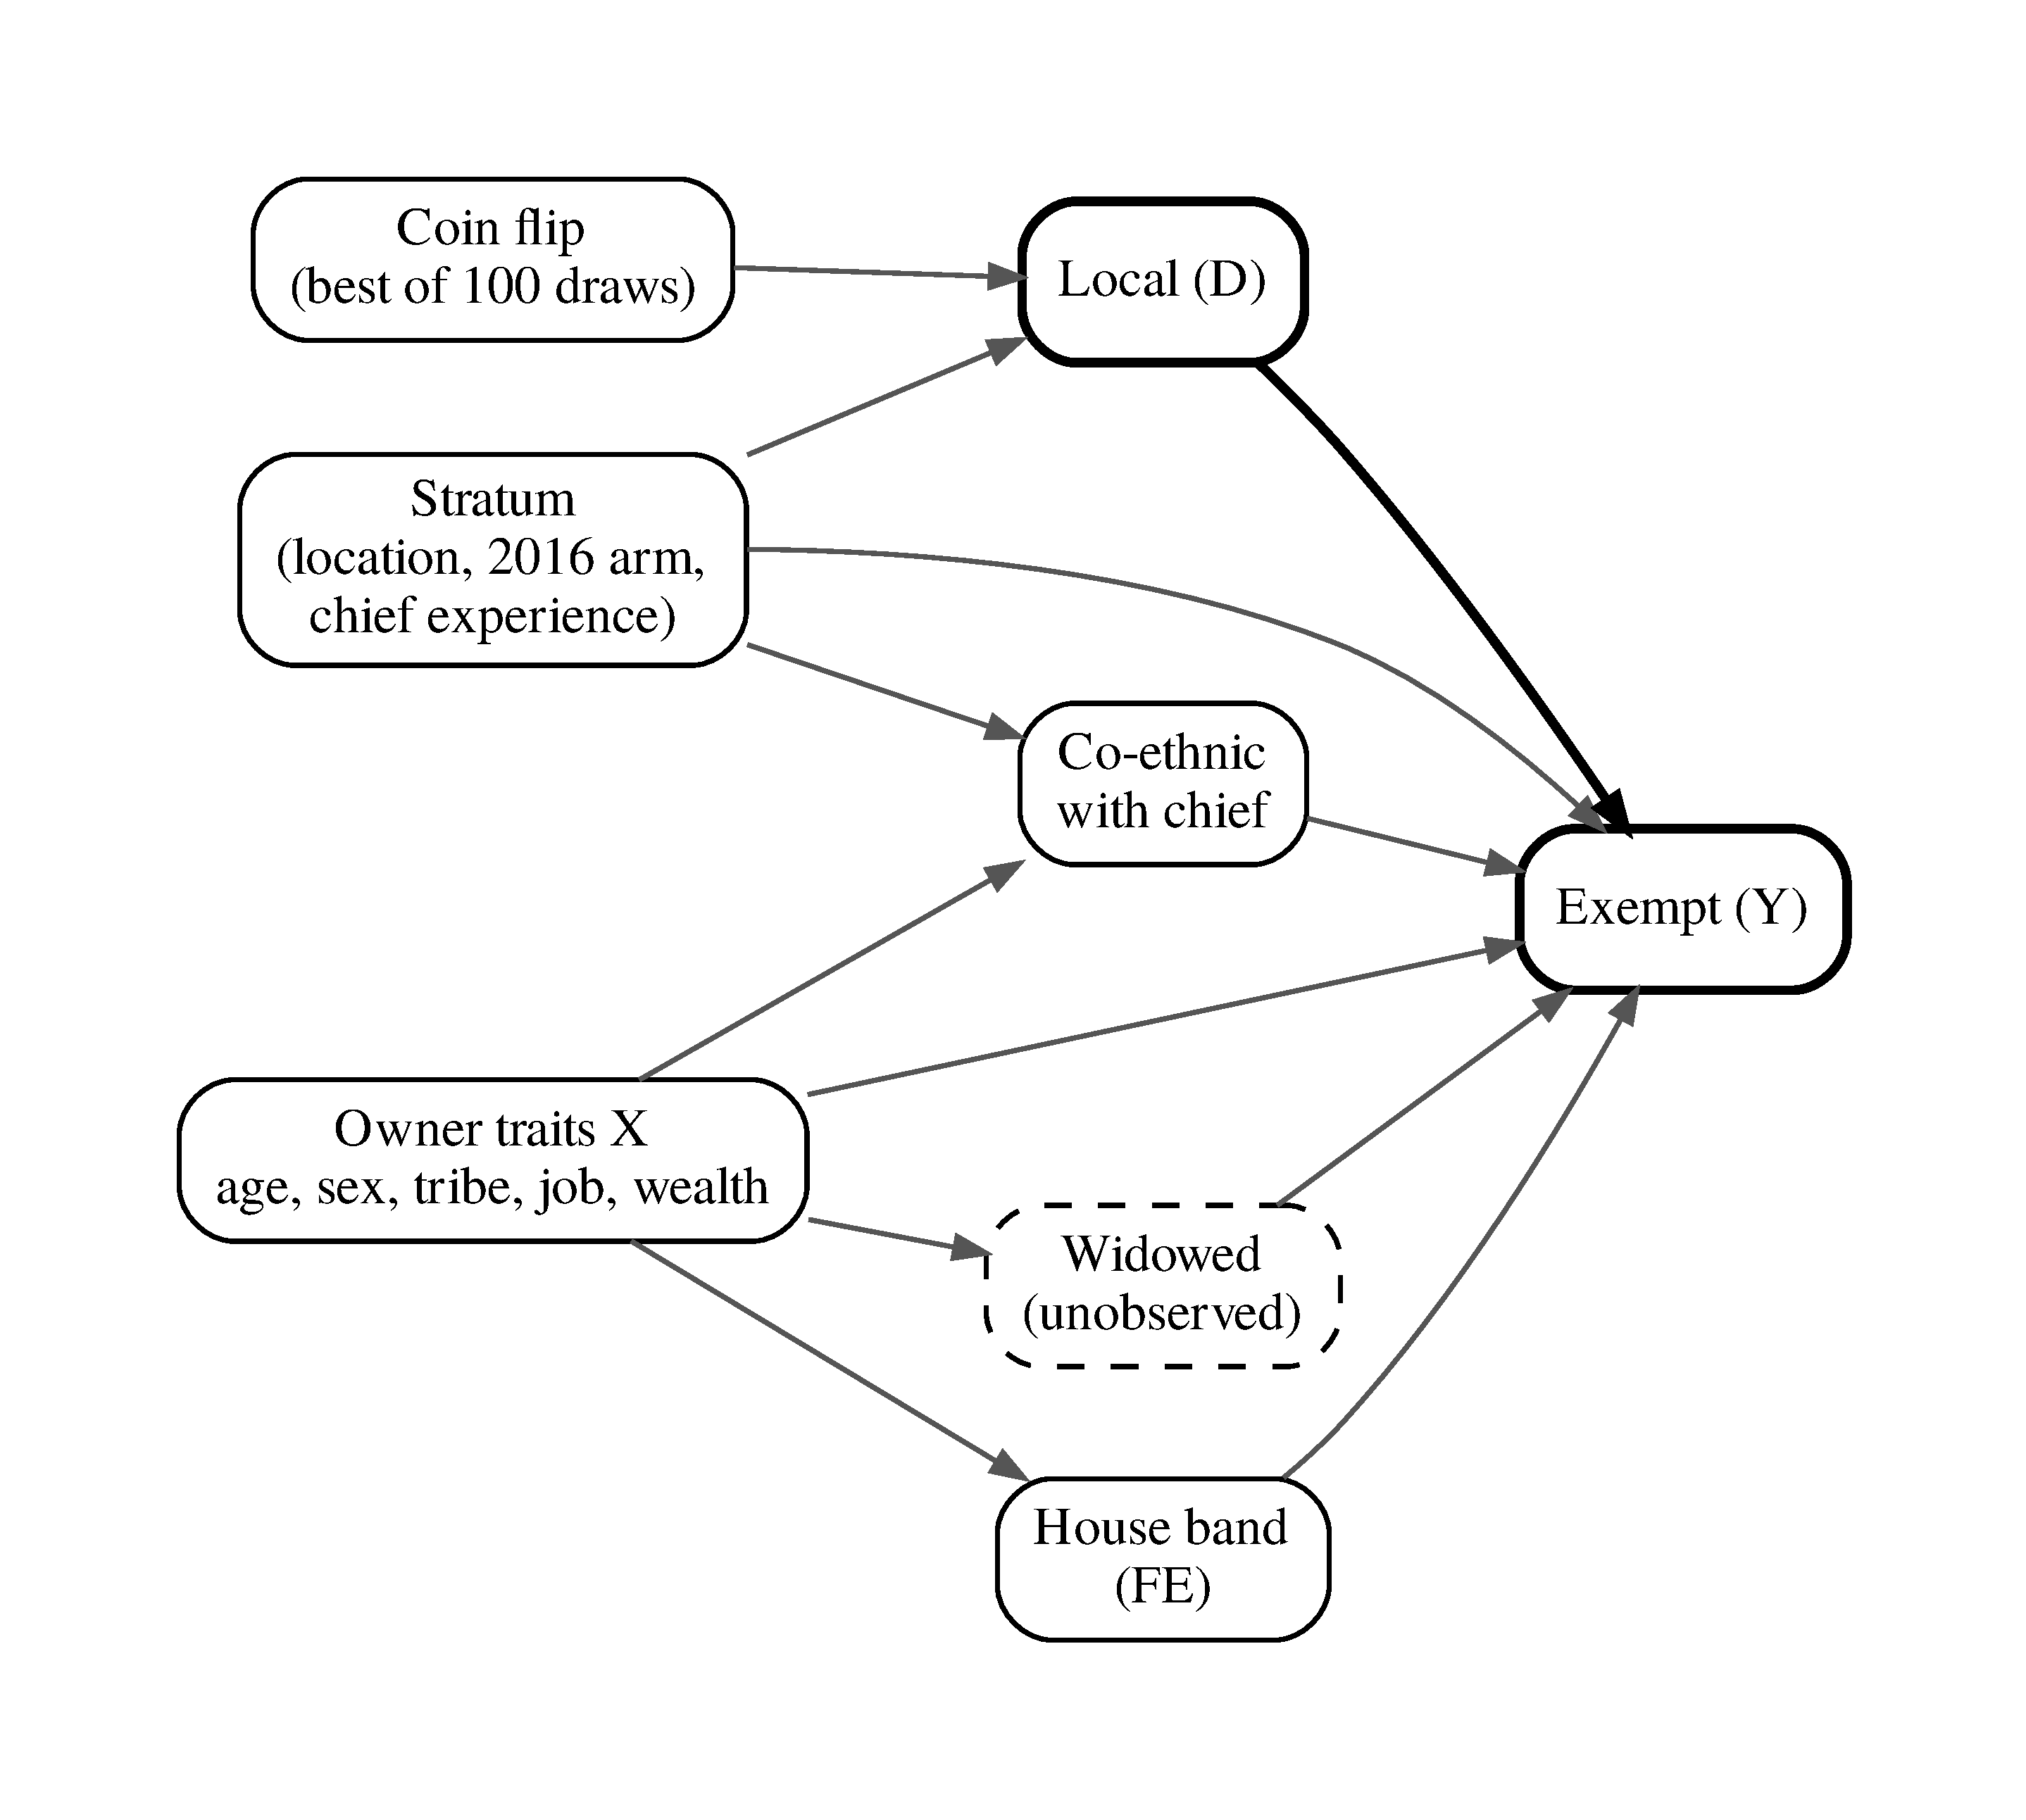
\includegraphics[width=\textwidth]{fig2a_dag1.pdf}\caption{DAG 1: the experiment}\end{subfigure}\hfill
\begin{subfigure}{0.46\textwidth}\centering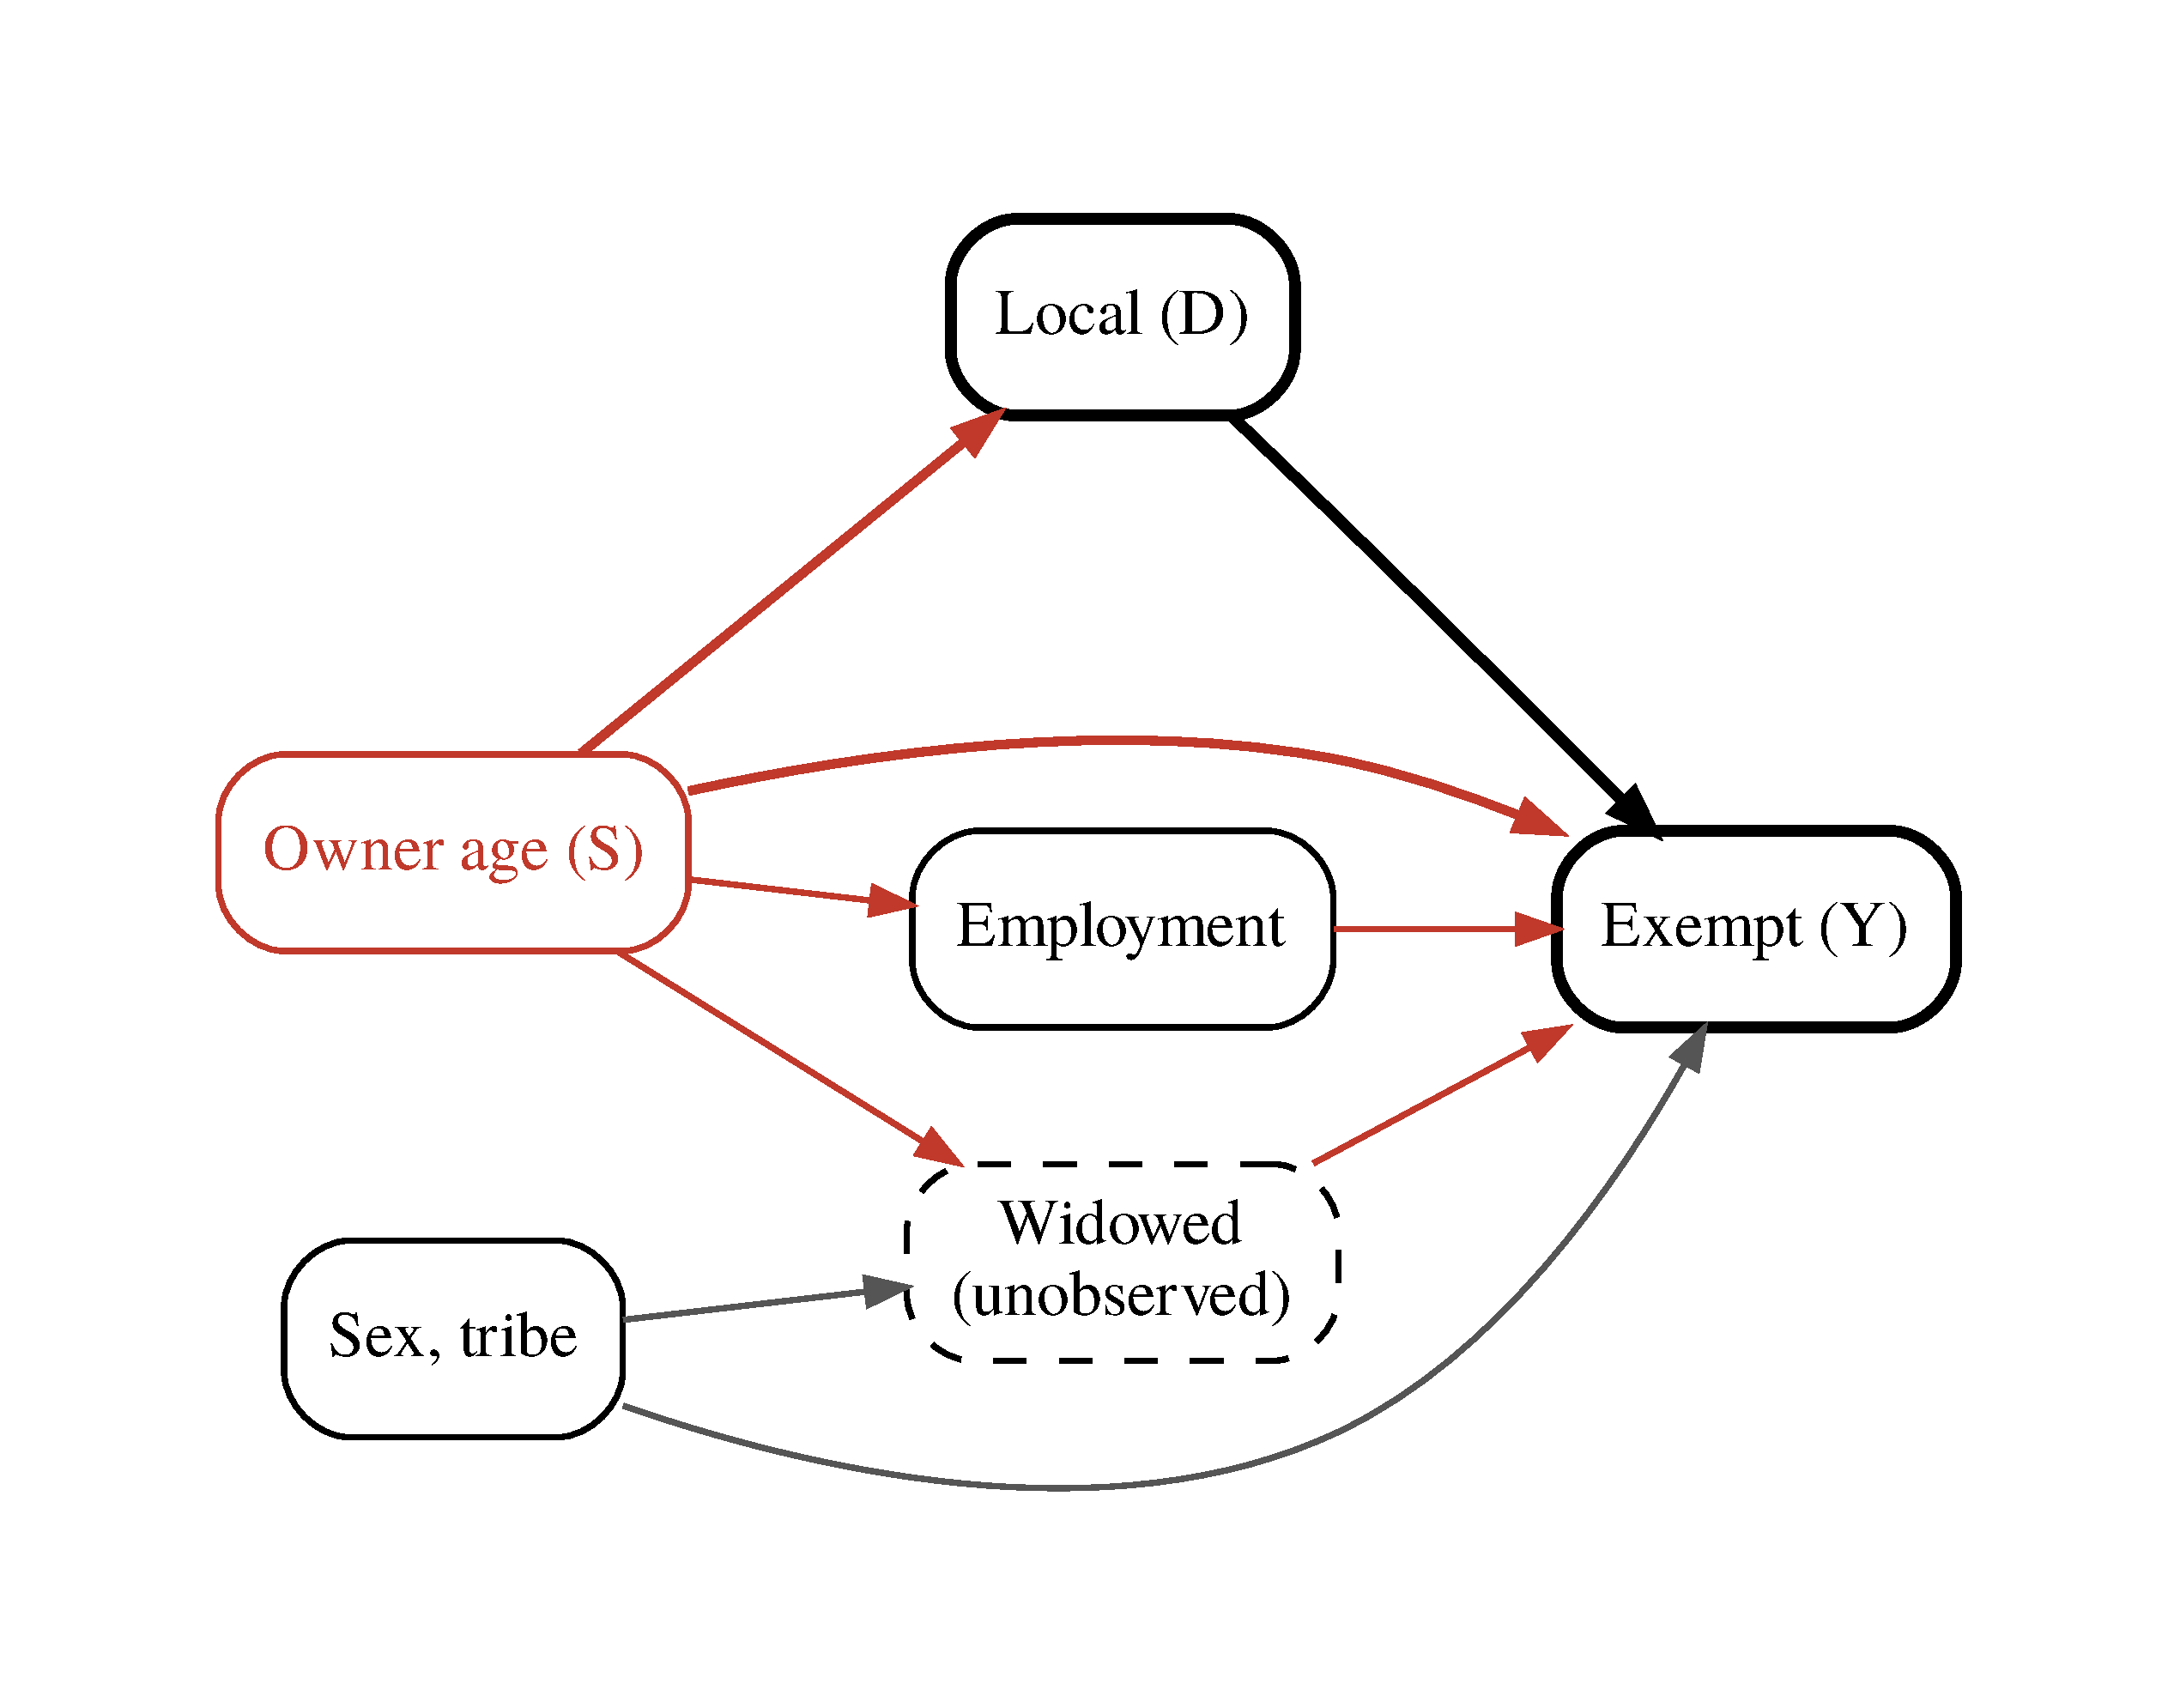
\includegraphics[width=\textwidth]{fig2b_dag2.pdf}\caption{DAG 2: selection on owner age $S$}\end{subfigure}\\[6pt]
\begin{subfigure}{0.62\textwidth}\centering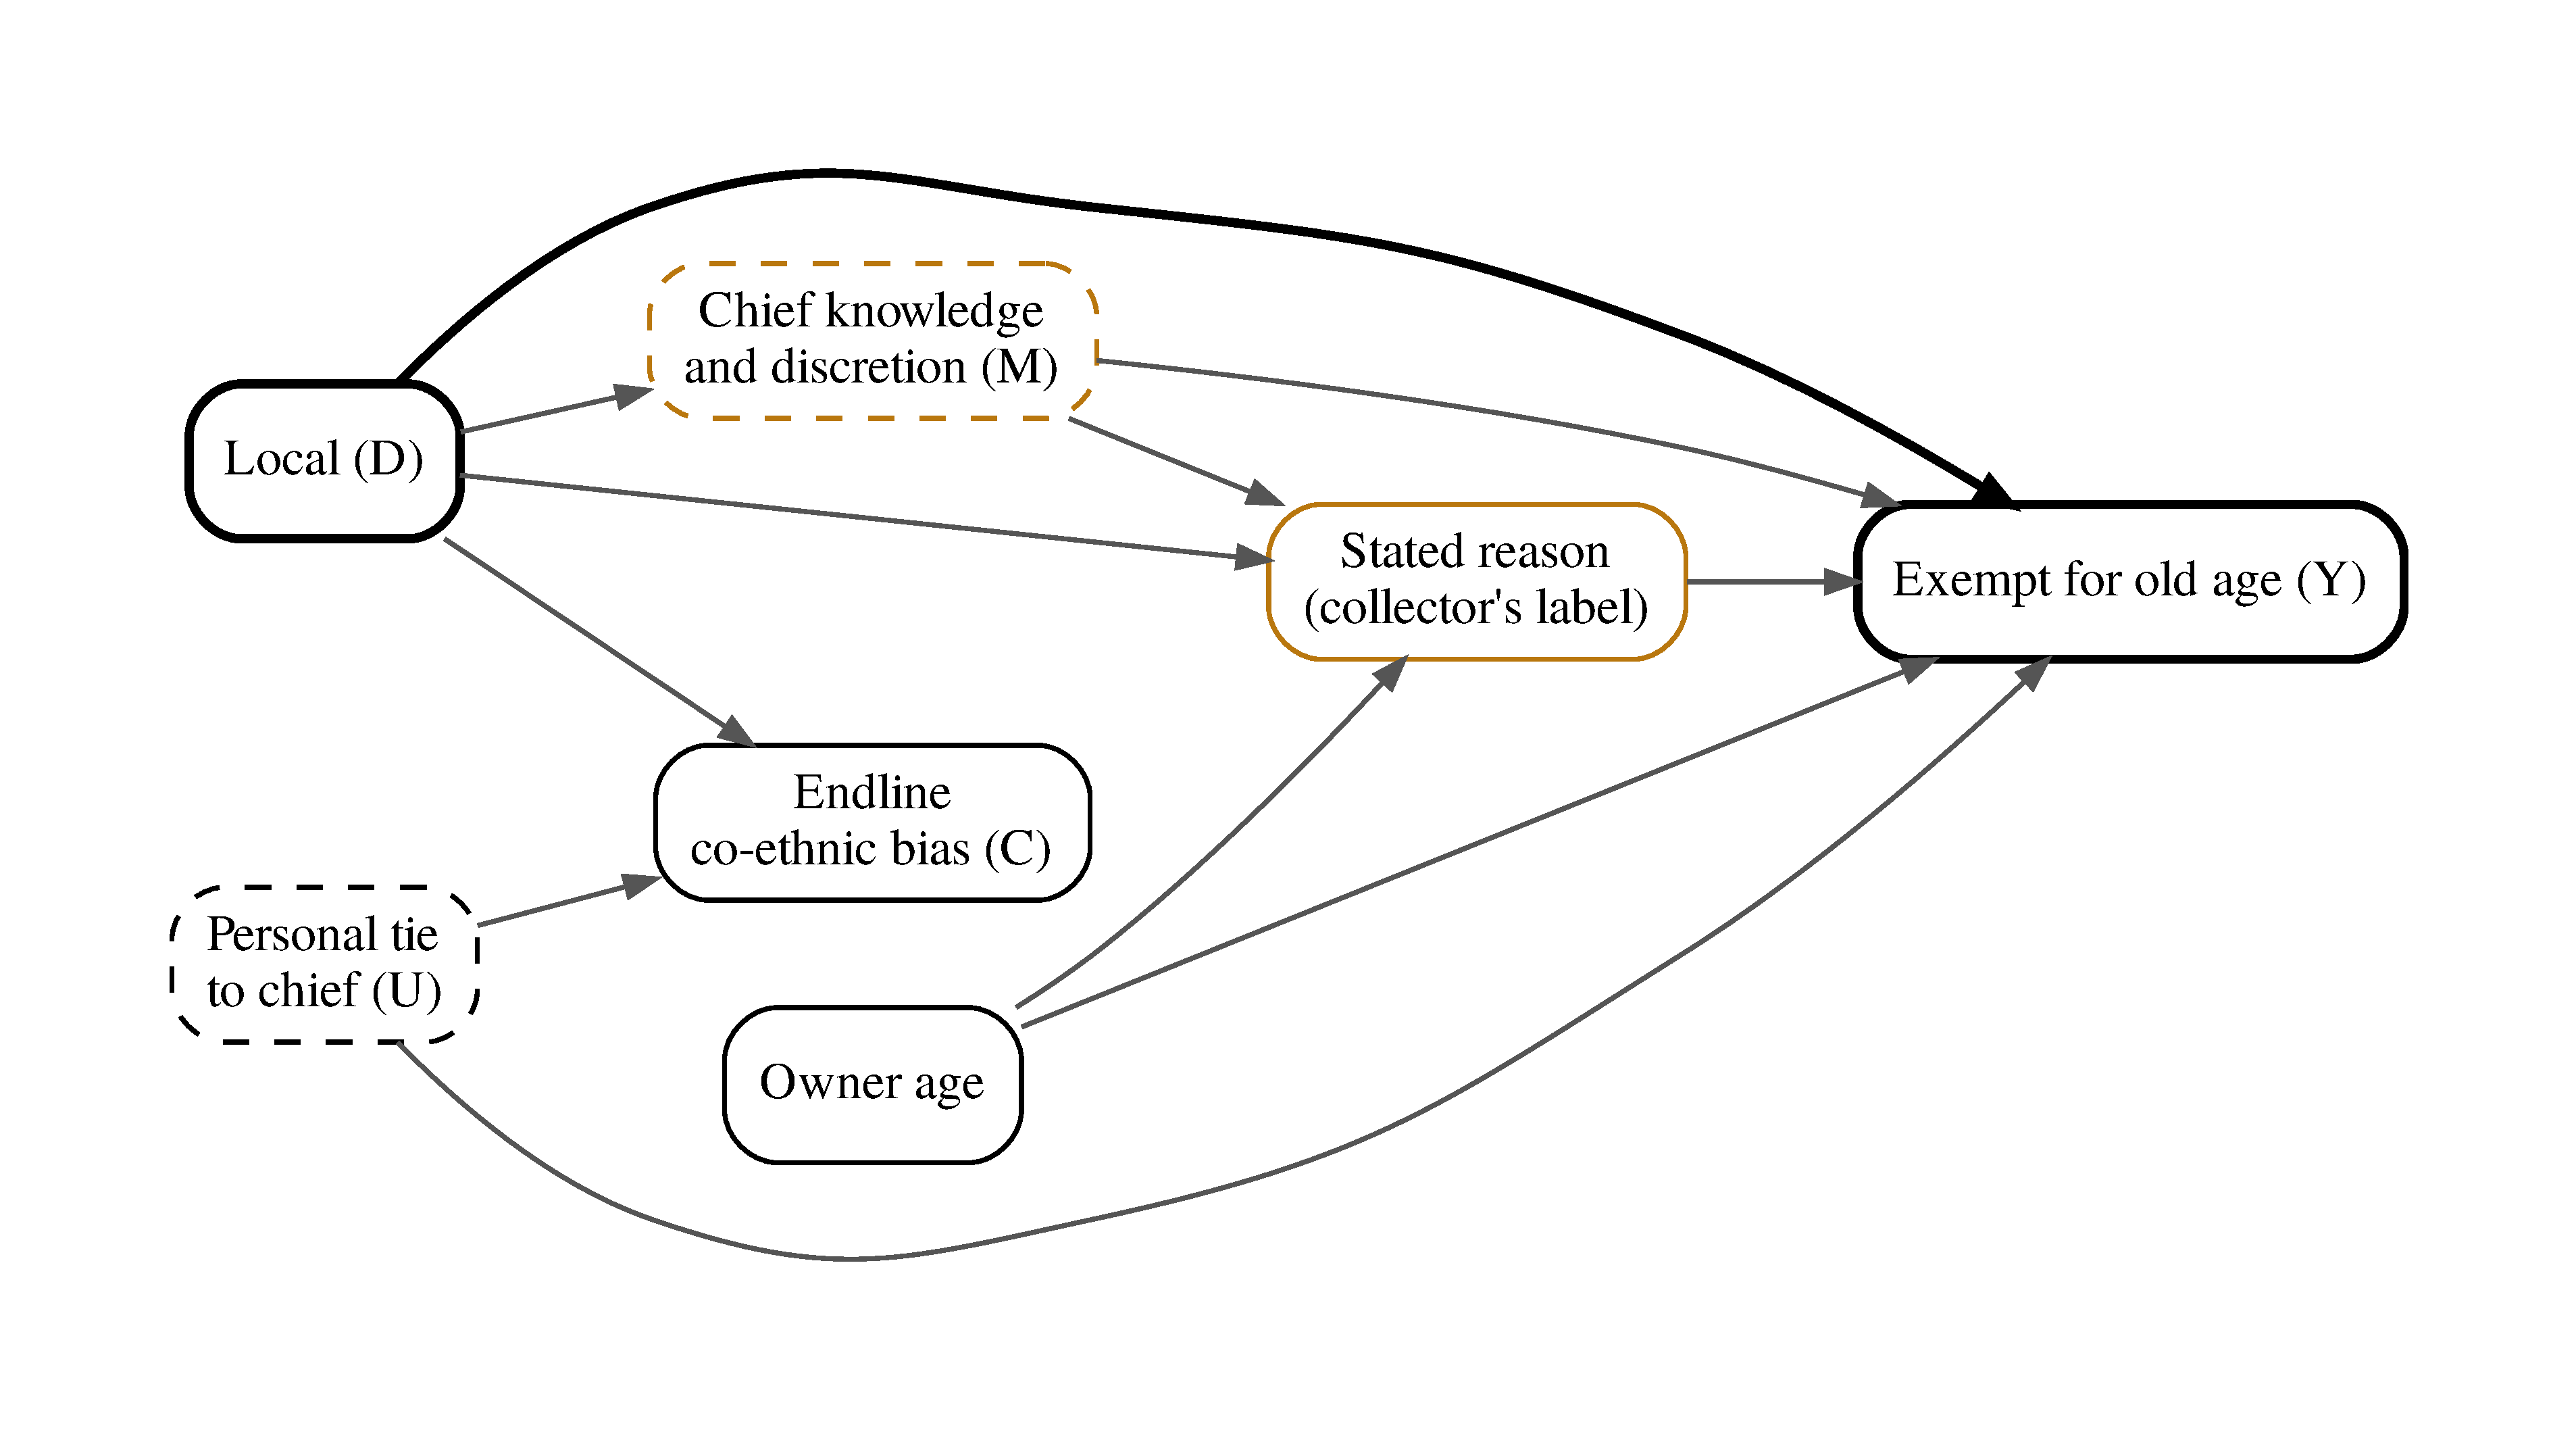
\includegraphics[width=\textwidth]{fig2c_dag3.pdf}\caption{DAG 3: mediators, the reason label and a collider}\end{subfigure}
\caption{Causal graphs. Bold arrows are the effect of interest; red arrows are back-door paths opened by selection on age; dashed nodes are unobserved.}\label{fig:dags}
\end{figure}

\paragraph{Randomization validity.} Table~\ref{tab:balance} and Figure~\ref{fig:balance} test balance. Among all 22,549 properties matched to the midline survey, Local and Central owners have the same age, sex, tribe, employment and housing; only distance to the centre differs ($+0.17$ km, $p=0.04$), and the joint test does not reject at 5\% ($p=0.08$). Chiefs are similar in age, education, tribe and tenure, though Local chiefs are less often women (one in twenty Central chiefs is a woman). The owner-linked sample is less balanced: Local owners are 1.3 years older, 4.3 points less often female and 8.9 points more often co-ethnic with the chief, and the joint test rejects ($p<0.01$). These differences are not in the population; they come from which properties end up with a recorded decision and a surveyed owner. Since old and male owners are exempted for different reasons, this is the main threat to the owner-linked estimates, and I address it in three ways: controls for owner traits (DAG~2), post-double-selection Lasso, and a sample that does not condition on the recorded decision.

\input{\tabpath/table2_balance.tex}

\begin{figure}[!htbp]\centering
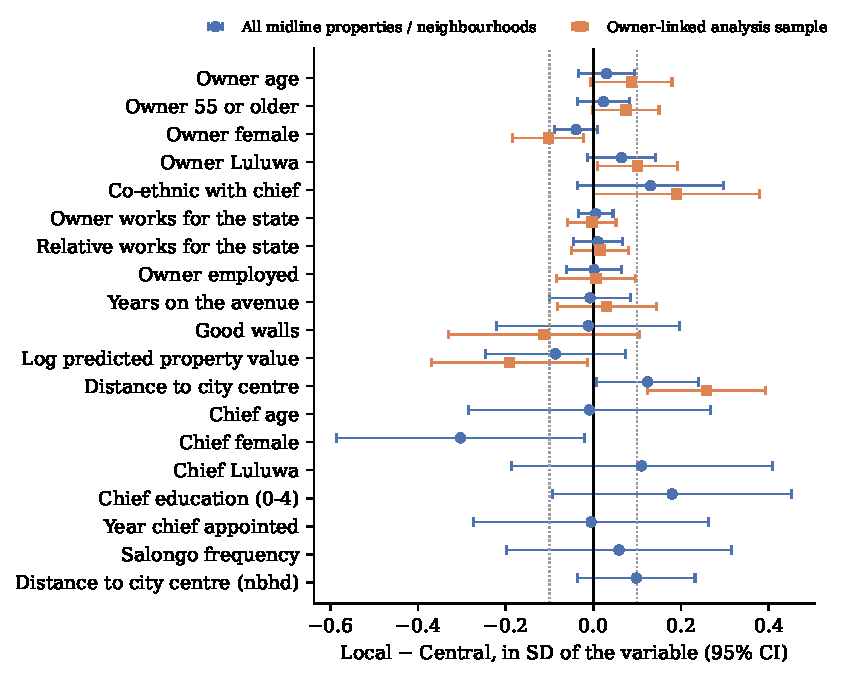
\includegraphics[width=0.66\textwidth]{fig3_balance.pdf}
\caption{Standardized Local--Central differences (stratum fixed effects, 95\% CI clustered by neighbourhood). Dotted lines mark $\pm0.1$ SD.}\label{fig:balance}
\end{figure}

\paragraph{Attrition.} Panel C of Table~\ref{tab:balance} shows that the share of properties with a recorded exemption decision (51\% in Central) is 3.1 points lower in Local ($p=0.41$), the midline match rate is the same ($-1.8$ points, $p=0.46$), and the share of registered properties that enter the owner-linked sample is 5.6 points higher in Local but not significantly so ($p=0.18$). Age bands are used equally in both arms ($p=0.34$).

\paragraph{SUTVA.} SUTVA requires that a property's exemption depends only on its own neighbourhood's collector. Spillovers are plausible: chiefs of adjacent neighbourhoods talk, and owners can compare. Figure~\ref{fig:network} draws the adjacency network of the experiment's neighbourhoods. Local and Central neighbourhoods are interleaved across the city, and 185 of 868 borders separate a Local from a Central neighbourhood, so the share of a neighbourhood's neighbours that are Local varies at random. Table~\ref{tab:spill} uses this variation. The share of Local neighbours has no effect on any exemption outcome in the pooled sample (all $p>0.24$), and adding it leaves the own-treatment coefficients unchanged. Among Central properties alone, more Local neighbours are associated with more exemptions in the owner-linked sample, which would bias $\beta$ towards zero if anything.

\begin{figure}[!htbp]\centering
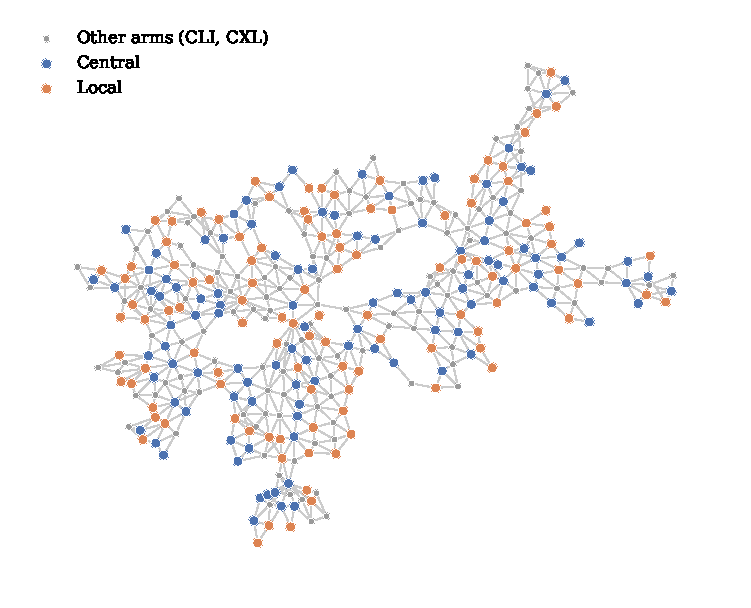
\includegraphics[width=0.62\textwidth]{fig4_network.pdf}
\caption{Adjacency network of the 351 experimental neighbourhoods (an edge is a shared border). Layout by graph distance, not geography.}\label{fig:network}
\end{figure}

\input{\tabpath/table3_spillover.tex}

% ===========================================================================
\section{Results}\label{sec:results}
% ===========================================================================

\subsection{Replication of the original estimates}

Table~\ref{tab:replication} reproduces the paper. Chief collection raises compliance by 2.3 points (SE 0.8, $N=28{,}872$, 221 clusters), the exact estimate in Table 4 of \citet{balan2022}. On the registered sample, chiefs raise exemptions by 3.9 points over a Central mean of 26.6\%. The rise comes from old-age exemptions (4.1 points, a third more than the Central mean of 12.2\%) and a small rise in disability exemptions, while widow exemptions do not move. The enumerator disagrees with Local collectors 1.2 points more often, not significantly. These are the numbers the authors read as chiefs applying the old-age rule more faithfully. The rest of the paper asks whether the additional old-age exemptions go to old owners.

\input{\tabpath/table4_replication.tex}

\subsection{Main estimates: more old-age labels, not more exemptions}

\input{\tabpath/table5_ate.tex}

Table~\ref{tab:ate} reports equation~\eqref{eq:ate} for nine outcomes in the owner-linked sample. In Panel A, chiefs raise old-age exemptions by 4.8 points ($p=0.02$), 37\% of the Central mean, and reduce widow exemptions by 2.7 points ($p=0.12$), so that total exemptions rise by an insignificant 1.9 points. Splitting old-age exemptions by legal eligibility, three quarters of the rise goes to owners aged 55 or older (3.6 points, column 5), which is consistent with the authors' reading. The remaining quarter is new: old-age exemptions for owners under 55 rise by 1.1 points ($p=0.01$), from 1.4\% to 2.5\%, an 82\% increase. Widow exemptions of male owners do not rise (column 7), and the combined discretionary measure rises by 0.7 points, not significantly. Column 9 is the cleanest test of favours because it does not use the reason the collector wrote down: exemptions of men under 55 who are not pensioners or disabled rise by only 0.6 points ($p=0.33$) on a 2.7\% base.

Panel B adds owner covariates. The estimate for discretionary old-age exemptions is unchanged (1.2 points, $p=0.01$), but the overall old-age effect falls from 4.8 to 2.6 points and loses significance. The drop is what DAG~2 predicts: in this sample Local owners are older and more often men, and controlling for age and sex removes the part of the gap that comes from who was sampled. The $R^2$ jumps from 0.07 to 0.20 for old-age exemptions and to 0.34 for any exemption, which says that owner traits, not the collector, explain most of who is exempted.

Figure~\ref{fig:byage} estimates the Local effect separately by age band. Chiefs raise old-age exemptions by 4--7 points in five of the six bands, including owners under 40 (4.7 points) and aged 50--54 (5.2 points), and lower widow exemptions in most of the same bands, so that the effect on any exemption is small in every band. Put together, Table~\ref{tab:ate} and Figure~\ref{fig:byage} say that chiefs grant exemptions to roughly the same owners as state agents, but write ``old age'' where state agents write ``widow''. One reading is that chiefs know who is a widow but find ``old age'' an easier label to defend, or that they treat elderly-looking widows as elderly. Either way, an audit that checks the stated reason would flag Local exemptions as discretionary when the owner would have been exempted anyway.

\begin{figure}[!htbp]\centering
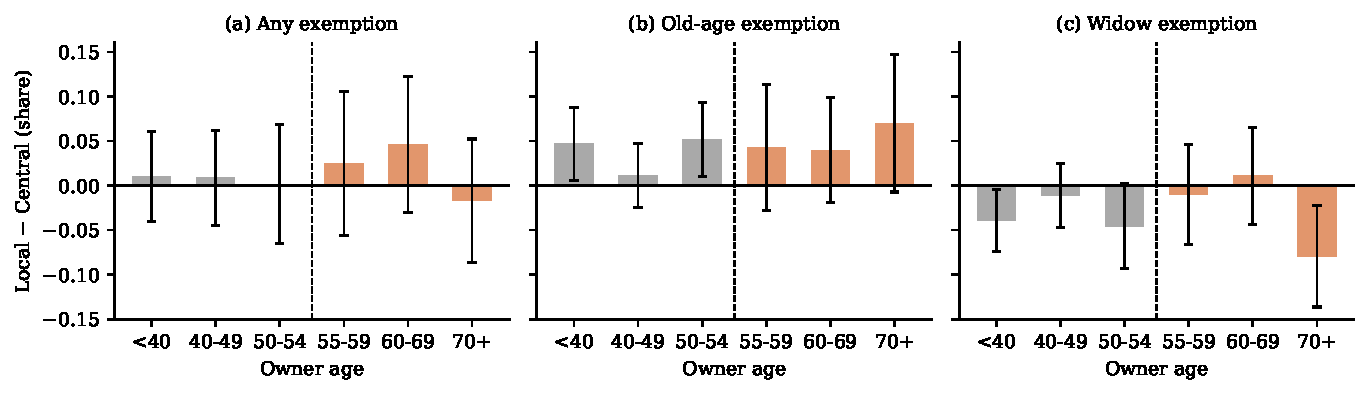
\includegraphics[width=\textwidth]{fig5_effect_by_age.pdf}
\caption{Local--Central difference by owner age band, from one regression per outcome with Local interacted with each band, band fixed effects and equation~\eqref{eq:ate} fixed effects (95\% CI clustered by neighbourhood). Grey bars: owners below the legal age.}\label{fig:byage}
\end{figure}

\paragraph{How big is it in money?} An extra 1.1 discretionary old-age exemptions per 100 properties at the periphery rate of about 2,250 CF is roughly \$17 of liability per 1,000 properties, a third of the \$53 per 1,000 properties that chiefs add in revenue \citep{balan2022}. Since only about 7\% of non-exempt owners pay, the expected revenue lost is near \$1 per 1,000 properties, and since total exemptions barely rise, even that may be an overstatement.

\subsection{Heterogeneity: OLS interactions}

Table~\ref{tab:het} estimates equation~\eqref{eq:het} with four moderators: owner 55 or older, female owner, co-ethnic with the chief, and a relative working for the state. If chiefs used exemptions as favours, the effect should be larger for co-ethnics or for politically connected households; if they knew the law better, it should be larger for eligible owners. None of the twelve interactions is significant. The co-ethnic interaction is negative for any exemption ($-4.5$ points, $p=0.28$), the opposite of favouritism, and it is close to zero for old-age exemptions. The relative-in-the-state interaction is positive (3.1 points for old-age exemptions) but imprecise ($p=0.18$). The main effects show the exemption rule clearly: being 55 or older raises the exemption rate by 36 points and being a woman by 33 points, so the legal criteria, not ethnicity or connections, sort owners.

\input{\tabpath/table6_heterogeneity.tex}

\subsection{Regularization: Ridge and Lasso}

The interactions in Table~\ref{tab:het} were chosen by me. Ridge and Lasso let the data choose among all 23 terms: Local, eleven owner covariates and their eleven interactions with Local. For the old-age outcome, after partialling out the fixed effects and standardizing, Ridge solves $\min_b \sum_i (\tilde y_i - \tilde x_i'b)^2 + \lambda\lVert b\rVert_2^2$ and Lasso replaces the penalty with $\lambda\lVert b\rVert_1$, with $\lambda$ chosen by 10-fold cross-validation with folds grouped by neighbourhood so that no neighbourhood is in both training and validation folds.

\begin{figure}[!htbp]\centering
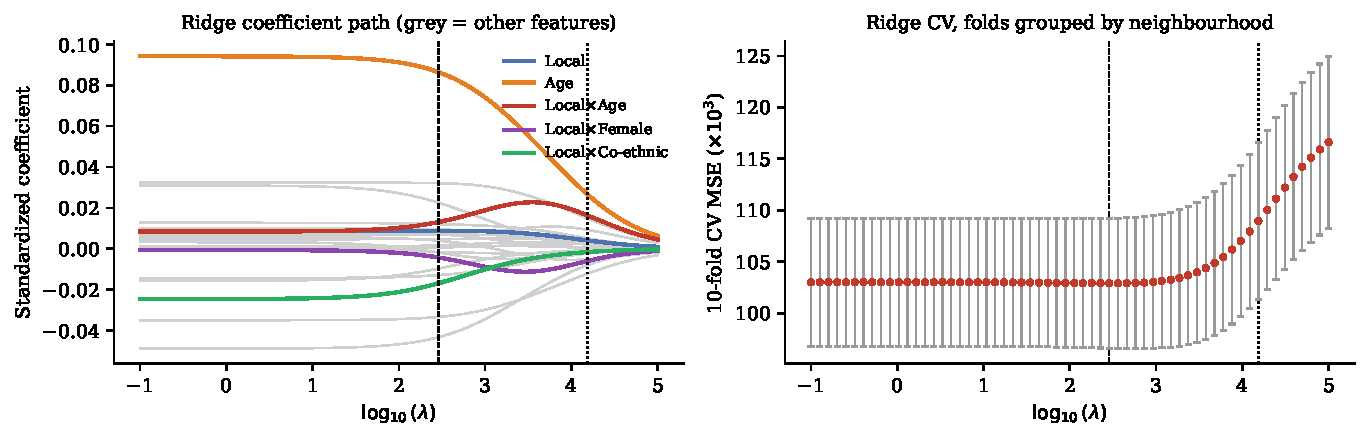
\includegraphics[width=\textwidth]{fig6a_ridge.pdf}
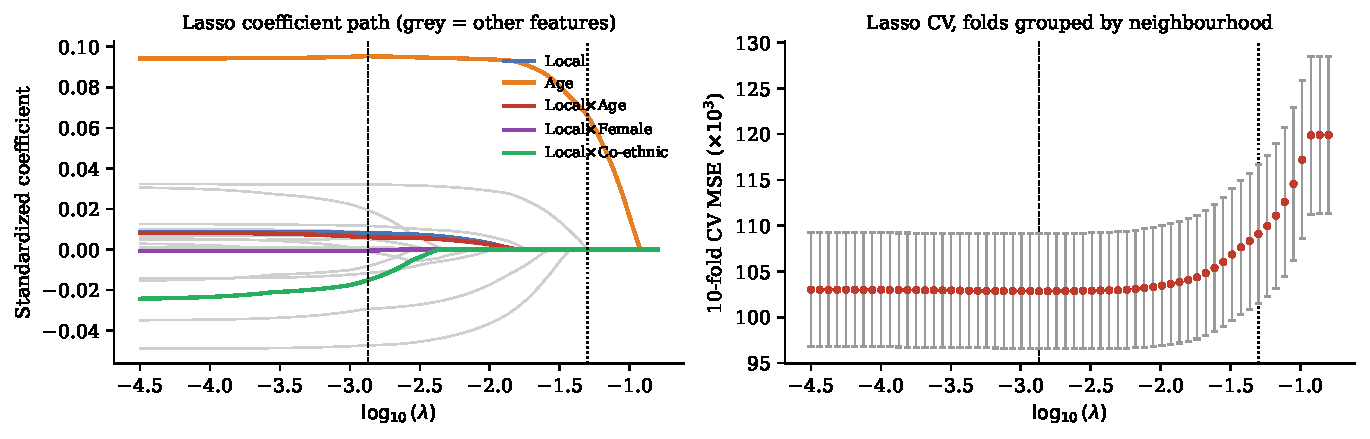
\includegraphics[width=\textwidth]{fig6b_lasso.pdf}
\caption{Ridge (top) and Lasso (bottom): coefficient paths and grouped 10-fold CV error ($\pm1$ SE). Dashed line: $\lambda_{min}$; dotted line: $\lambda_{1se}$. Outcome: exempt for old age.}\label{fig:reg}
\end{figure}

\input{\tabpath/table7_regularization.tex}

Figure~\ref{fig:reg} and Table~\ref{tab:reg} give the same answer as OLS. Age dominates every path; Ridge shrinks all interactions towards zero as $\lambda$ rises, and in the Lasso path Age is the last coefficient to leave. At $\lambda_{min}$ the Lasso keeps 19 terms, but the interactions it keeps are tiny (Local$\times$Age 0.006, Local$\times$Co-ethnic $-0.015$ standard deviations), and the CV error at $\lambda_{min}$ is no lower than at $\lambda_{1se}$ by more than its standard error. At $\lambda_{1se}$ only age and one other term survive and Local itself is dropped. The interactions therefore add no predictive power, which tells us more than the insignificant OLS coefficients: it is not that the heterogeneity is imprecisely estimated but that, in a linear model, there is little to find. The bottom panel of Table~\ref{tab:reg} uses the Lasso for a different job, selecting controls for the ATE by post-double selection \citep{chernozhukov2018}. The selected controls give a discretionary old-age effect of 1.2 points ($p=0.02$), the same as Table~\ref{tab:ate}.

\subsection{Robustness}

Table~\ref{tab:robust} checks the main estimates. The discretionary old-age effect is significant at every age cut-off from 50 to 65 (rows 2--4), grows as the cut-off rises because more borderline owners are counted, survives dropping banded ages (row 5, $p=0.05$), removing fixed effects (rows 6--7), a logit (row 9), controlling for neighbours' treatment (row 10) and owner covariates (row 11). Collapsing to neighbourhood means (row 8) gives the same point estimate with a larger standard error, as expected with 197 noisy cluster means. Row 13 addresses selection: in all 12,305 midline-matched properties with owner age and sex, counting an unrecorded decision as ``not exempt'', discretionary old-age exemptions still rise (0.4 points, $p=0.03$) while total exemptions do not. Randomization inference, which re-draws assignment within strata 2,000 times and needs no asymptotics with 197 clusters, gives $p=0.009$ for discretionary old-age exemptions, $p=0.045$ for old-age exemptions, and $p=0.60$ for any exemption (Figure~\ref{fig:ri}). The finding that chiefs re-label but do not add exemptions is robust; the finding that chiefs add old-age exemptions overall is less so once the sample composition is held fixed.

\input{\tabpath/table8_robustness.tex}

\begin{figure}[!htbp]\centering
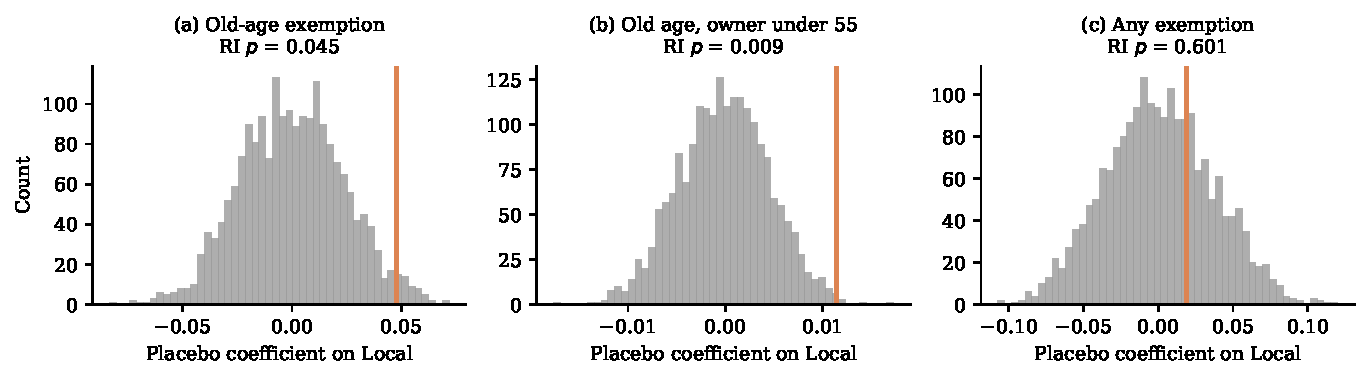
\includegraphics[width=\textwidth]{fig7_ri.pdf}
\caption{Randomization inference: distribution of the Local coefficient under 2,000 within-stratum re-assignments (seed 1465). The orange line is the actual estimate.}\label{fig:ri}
\end{figure}

\subsection{Tree-based models}\label{sec:trees}

Trees ask a different question from equation~\eqref{eq:ate}: which features best predict exemption, and does Local matter once nonlinearities and interactions are allowed? I predict $Y=$ any exemption (and, in the last two columns of Table~\ref{tab:ml}, old-age exemption) from 16 pre-determined features including Local, holding out 20\% of neighbourhoods (41 neighbourhoods, 1,289 properties) for testing and tuning everything by 10-fold CV grouped by neighbourhood inside the training set. A regression tree partitions the feature space into regions $R_m$ and predicts the region mean, choosing splits to minimize $\sum_m\sum_{i\in R_m}(y_i-\bar y_{R_m})^2$ and pruning with a cost $\alpha|T|$ for the number of leaves. Bagging averages 500 trees grown on bootstrap samples; the random forest also samples $m$ of the 16 features at each split to decorrelate the trees; boosting fits 351 small trees ($d=3$) in sequence, each to the residuals of the previous ones, shrunk by $\lambda=0.01$.

\begin{figure}[!htbp]\centering
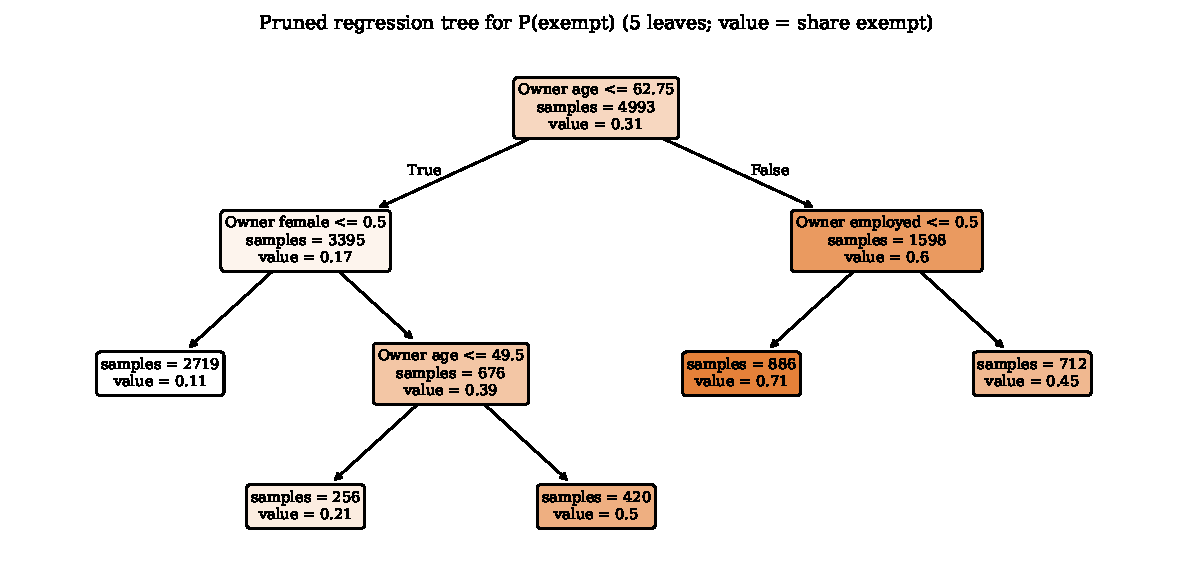
\includegraphics[width=0.92\textwidth]{fig8_tree.pdf}
\caption{Pruned regression tree for any exemption, owner-linked training sample. Complexity chosen by grouped 10-fold CV (1-SE rule). ``Owner female $\le 0.5$'' means a male owner; ``Owner employed $\le 0.5$'' means not employed.}\label{fig:tree}
\end{figure}

The pruned tree (Figure~\ref{fig:tree}) has five leaves and never splits on Local. Its first split is at age 62.75, not 55: owners older than that are exempted 60\% of the time, and 71\% if they do not work. Below 62.75, men are exempted 11\% of the time and women 39\%, and women aged 49.5 or more 50\%, which is the widow exemption showing up as an interaction between sex and age. Two thresholds stand out. The age split well above the legal 55 says that collectors in both arms treat 55--62-year-olds as only partly eligible, so the law's cut-off is not what sorts owners in practice. The sex-by-age leaf says that the widow and old-age rules overlap for older women, which is exactly where a collector can choose the label. The tree finds no Local split because the 2--5 point Local effects are tiny next to these 40--60 point gaps.

\input{\tabpath/table9_ml_errors.tex}

\begin{figure}[!htbp]\centering
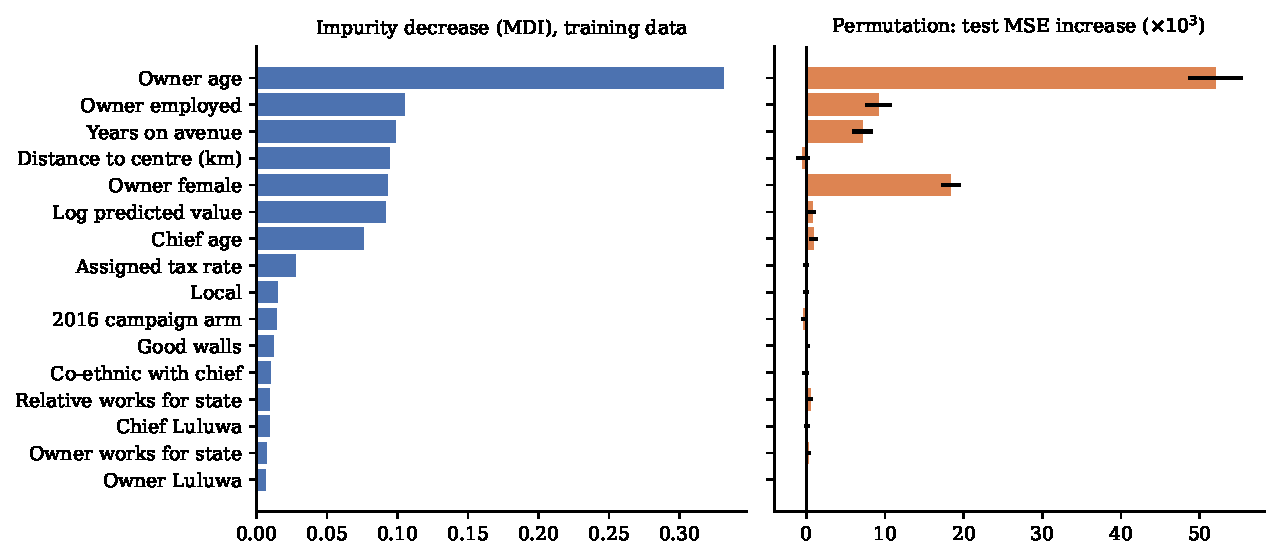
\includegraphics[width=0.9\textwidth]{fig9_rf_importance.pdf}
\caption{Random forest ($m=4$, 500 trees) for any exemption. Left: mean decrease in impurity on the training data. Right: rise in test MSE when a feature is permuted (20 repeats, $\pm1$ SD).}\label{fig:imp}
\end{figure}

Table~\ref{tab:ml} compares test errors. All models cut the error of the mean by 30--36\%. Boosting is best (test MSE 0.138), followed by the random forest (0.140), OLS (0.142), bagging (0.144) and the pruned tree (0.149). The ranking is the textbook one: averaging many deep trees beats one tree, decorrelating them by sampling $m=4$ features beats bagging, whose trees all split first on age, and the out-of-bag errors (0.143 and 0.147) track the test errors. But the gains over OLS are small, because the structure is simple: an age threshold and a sex-age interaction. For old-age exemptions boosting and the forest again do best, and bagging also beats OLS.

Figure~\ref{fig:imp} reads the random forest. Owner age dominates both measures: permuting it raises test MSE by 0.052, more than twice the next feature, owner sex (0.018). Employment (0.009) and years on the avenue (0.007) follow. Distance to the centre ranks fourth by impurity but its permutation importance is zero, the known bias of impurity measures towards continuous features with many split points. Local ranks ninth by impurity and its permutation importance is zero ($-0.0001$): shuffling who collects does not hurt the forest's predictions at all. Co-ethnicity with the chief and the chief's tribe are also near zero on both measures, which repeats the result of Table~\ref{tab:het} without imposing linearity.

\begin{figure}[!htbp]\centering
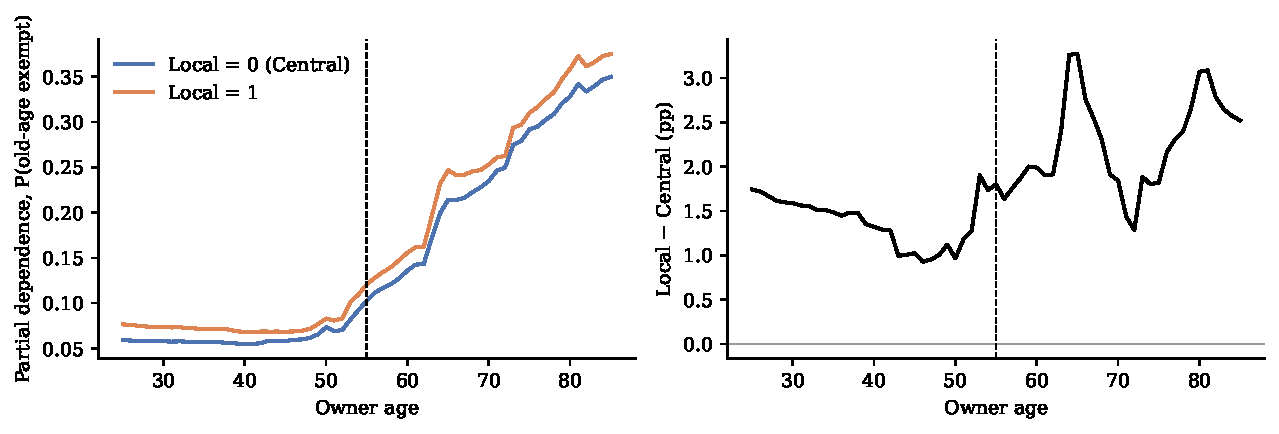
\includegraphics[width=0.9\textwidth]{fig10_pdp.pdf}
\caption{Partial dependence of the random-forest prediction of old-age exemption on owner age, with Local set to 0 and to 1 for every property (left), and their difference (right).}\label{fig:pdp}
\end{figure}

Finally, Figure~\ref{fig:pdp} uses a random forest trained on old-age exemptions to ask where Local shifts the prediction. With Local switched on for every property, the predicted probability of an old-age exemption is 1--2 points higher below 55 and 2--3 points higher above it. The forest is a prediction model and its gap is not a causal estimate with a standard error, but it agrees with Figure~\ref{fig:byage}: the Local shift in old-age labels is spread across all ages rather than concentrated just below the threshold, where a favour to a ``nearly old'' owner would show up.


% ===========================================================================
\section{Conclusion}\label{sec:conc}
% ===========================================================================

I asked whether city chiefs, given the job of collecting the property tax, grant more exemptions that the law does not allow. They do not grant many more exemptions. They do record more of them as old-age exemptions, including for owners well below the legal age, and fewer as widow exemptions, so that a reason-based audit finds an 82\% rise in discretionary old-age exemptions while a reason-free measure finds none. The effect does not vary with co-ethnicity, political connections, age or sex in any model I estimate, linear or not. For the debate on delegating taxation to local elites, this is reassuring on favouritism but sobering on measurement: the labels collectors write are themselves an outcome of who collects. The authors' finding that chiefs exempt the elderly more often is partly a finding about labels. Against chiefs' revenue gain, the money at stake in discretionary exemptions is small, roughly a third of the gain in liability terms and much less in expected payments.

\section{Future Steps}

Project Two will estimate heterogeneity with honest causal forests clustered by neighbourhood \citep{wager2018,athey2019} and test it with the best-linear-projection and sorted-group methods of \citet{chernozhukov2018b}, on the three outcomes that matter here: the old-age label, the widow label and the reason-free measure. I will add the endline bribe and the endline co-ethnic-bias questions as outcomes (not moderators, per DAG~3), use the 2017 household baseline to obtain owner age before treatment for about a fifth of the sample, and bound the composition effect in the owner-linked sample with Lee bounds.

% ===========================================================================
\begin{thebibliography}{99}\small\setlength{\itemsep}{1pt}
\bibitem[Acemoglu et al.(2014)]{acemoglu2014} Acemoglu, D., Reed, T., and Robinson, J. A. (2014). Chiefs: Economic development and elite control of civil society in Sierra Leone. \textit{Journal of Political Economy}, 122(2), 319--368.
\bibitem[Alatas et al.(2012)]{alatas2012} Alatas, V., Banerjee, A., Hanna, R., Olken, B. A., and Tobias, J. (2012). Targeting the poor: Evidence from a field experiment in Indonesia. \textit{American Economic Review}, 102(4), 1206--1240.
\bibitem[Anderson et al.(2015)]{anderson2015} Anderson, S., Francois, P., and Kotwal, A. (2015). Clientelism in Indian villages. \textit{American Economic Review}, 105(6), 1780--1816.
\bibitem[Athey et al.(2019)]{athey2019} Athey, S., Tibshirani, J., and Wager, S. (2019). Generalized random forests. \textit{Annals of Statistics}, 47(2), 1148--1178.
\bibitem[Bal\'an et al.(2022)]{balan2022} Bal\'an, P., Bergeron, A., Tourek, G., and Weigel, J. L. (2022). Local elites as state capacity: How city chiefs use local information to increase tax compliance in the Democratic Republic of the Congo. \textit{American Economic Review}, 112(3), 762--797. Data: \href{https://doi.org/10.3886/E147561V1}{doi.org/10.3886/E147561V1}.
\bibitem[Baldwin(2016)]{baldwin2016} Baldwin, K. (2016). \textit{The Paradox of Traditional Chiefs in Democratic Africa}. Cambridge University Press.
\bibitem[Bardhan and Mookherjee(2006)]{bardhan2006} Bardhan, P., and Mookherjee, D. (2006). Pro-poor targeting and accountability of local governments in West Bengal. \textit{Journal of Development Economics}, 79(2), 303--327.
\bibitem[Basurto et al.(2020)]{basurto2020} Basurto, M. P., Dupas, P., and Robinson, J. (2020). Decentralization and efficiency of subsidy targeting: Evidence from chiefs in rural Malawi. \textit{Journal of Public Economics}, 185, 104047.
\bibitem[Besley and Persson(2009)]{besley2009} Besley, T., and Persson, T. (2009). The origins of state capacity: Property rights, taxation, and politics. \textit{American Economic Review}, 99(4), 1218--1244.
\bibitem[Besley and Persson(2014)]{besley2014} Besley, T., and Persson, T. (2014). Why do developing countries tax so little? \textit{Journal of Economic Perspectives}, 28(4), 99--120.
\bibitem[Burgess et al.(2015)]{burgess2015} Burgess, R., Jedwab, R., Miguel, E., Morjaria, A., and Padr\'o i Miquel, G. (2015). The value of democracy: Evidence from road building in Kenya. \textit{American Economic Review}, 105(6), 1817--1851.
\bibitem[Chernozhukov et al.(2018a)]{chernozhukov2018} Chernozhukov, V., Chetverikov, D., Demirer, M., Duflo, E., Hansen, C., Newey, W., and Robins, J. (2018a). Double/debiased machine learning for treatment and structural parameters. \textit{Econometrics Journal}, 21(1), C1--C68.
\bibitem[Chernozhukov et al.(2018b)]{chernozhukov2018b} Chernozhukov, V., Demirer, M., Duflo, E., and Fern\'andez-Val, I. (2018b). Generic machine learning inference on heterogeneous treatment effects in randomized experiments. NBER Working Paper 24678.
\bibitem[Fisman et al.(2017)]{fisman2017} Fisman, R., Paravisini, D., and Vig, V. (2017). Cultural proximity and loan outcomes. \textit{American Economic Review}, 107(2), 457--492.
\bibitem[Khan et al.(2016)]{khan2016} Khan, A. Q., Khwaja, A. I., and Olken, B. A. (2016). Tax farming redux: Experimental evidence on performance pay for tax collectors. \textit{Quarterly Journal of Economics}, 131(1), 219--271.
\bibitem[Olken(2007)]{olken2007} Olken, B. A. (2007). Monitoring corruption: Evidence from a field experiment in Indonesia. \textit{Journal of Political Economy}, 115(2), 200--249.
\bibitem[Olken and Pande(2012)]{olken2012} Olken, B. A., and Pande, R. (2012). Corruption in developing countries. \textit{Annual Review of Economics}, 4, 479--509.
\bibitem[Pedregosa et al.(2011)]{sklearn} Pedregosa, F., et al. (2011). Scikit-learn: Machine learning in Python. \textit{Journal of Machine Learning Research}, 12, 2825--2830.
\bibitem[Seabold and Perktold(2010)]{statsmodels} Seabold, S., and Perktold, J. (2010). Statsmodels: Econometric and statistical modeling with Python. \textit{Proceedings of the 9th Python in Science Conference}.
\bibitem[Wager and Athey(2018)]{wager2018} Wager, S., and Athey, S. (2018). Estimation and inference of heterogeneous treatment effects using random forests. \textit{Journal of the American Statistical Association}, 113(523), 1228--1242.
\end{thebibliography}

% ===========================================================================
\appendix
\sloppy
\section{Data Construction and Reproduction}\label{app:data}
% ===========================================================================

All code is at \href{https://github.com/tsuning0905/MA_ECON1465}{github.com/tsuning0905/MA\_ECON1465}; running \texttt{python 00\_master/00\_master.py} rebuilds every table and figure in this paper from the raw files in \texttt{0\_RawData/}, which are never modified. The steps are:
\begin{enumerate}[leftmargin=*,itemsep=0pt]
\item \texttt{01\_preanalysis/01a\_data\_construction.py} ports the authors' \texttt{2\_Data\_Construction.do} to Python. It unzips the midline survey into \texttt{data\_intermediate/}, merges fliers, strata, assignment, registration, tax roll, midline and receipts by property id, builds \texttt{taxes\_paid} and \texttt{bribe\_combined} as in the do-file, cleans owner age (bands set to mid-points), sex, tribe and job, drops villas and pilot neighbourhoods, and fills missing campaign dates. It reproduces Table 4, column 1 to the third decimal.
\item \texttt{01\_preanalysis/01\_preanalysis.py} keeps the 221 Central and Local neighbourhoods; builds exemption indicators by \texttt{why\_exempt} (2 old age, 5 widow, 3 pension, 4 disability, others), the discretionary and reason-free measures at cut-offs 50/55/60/65, owner covariates (codes 88, 97--99, 8888, 9999 set to missing; age kept in 18--105), co-ethnicity with the chief named on the property's tax letter using the pre-randomization chief survey, distance to the centre, the authors' predicted property value, and the share of adjacent neighbourhoods assigned to Local. It writes \texttt{final\_property.csv.gz}, \texttt{final\_neighbourhood.csv} and a variable dictionary.
\item \texttt{02\_analysis/02\_analysis.py} produces Tables 1--9 (\texttt{.tex}, \texttt{.csv}, \texttt{.xlsx}) and Figures 1--10 (\texttt{.pdf}, \texttt{.png}) in \texttt{03\_output/}, in the order of this paper. Every random step uses seed 1465. Regressions use statsmodels \citep{statsmodels}; Ridge, Lasso and tree models use scikit-learn \citep{sklearn}; DAGs are drawn with Graphviz.
\end{enumerate}
In regressions, missing controls are set to the sample mean with a missing indicator. Properties whose campaign date falls outside the authors' two-month windows (4\% of the registered sample) drop out of fixed-effect regressions, as in the original code.

\end{document}
